Let
\begin{align}
   \vec{A} = \myvec{3\\6\\9} , \vec{B} = \myvec{10\\20\\30}, \vec{C} = \myvec{25\\-41\\5} 
\end{align}

\begin{align}
     (\vec{B}-\vec{A})^\top(\vec{C}-\vec{A})&=\myvec{7\ 14\ 21}\myvec{22\\-47\\-4}
     \\
& = -521 \ne 0
\\
     (\vec{A}-\vec{B})^\top(\vec{C}-\vec{B})&=\myvec{-7\ -14\ -21}\myvec{15\\-61\\-25}
\\
&= 1274 \ne 0
\\
(\vec{A}-\vec{B})^\top(\vec{C}-\vec{B})&=\myvec{-7\ -14\ -21}\myvec{15\\-61\\-25}
\\
&= 3397 \ne 0 
\end{align}
Hence, $\triangle ABC$ is not right angled as can be seen in Fig.          \ref{vectors/july/2/6/Figure}.
%
\begin{figure}[!h]
         \centering
         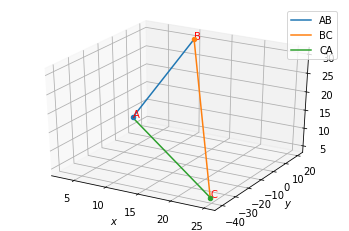
\includegraphics[width=\columnwidth]{solutions/july/2/6/Figures/Figure.png}
         \caption{Plot of the triangle}
         \label{vectors/july/2/6/Figure}
\end{figure}
